\documentclass{beamer}
\date{April 14, 2025}

\title{Numerical Approaches to the Heat Equation}
\author{Andrew Shea}
\usetheme{Madrid}
\begin{document}
\frame{\titlepage}

\begin{frame}{Introduction}
The heat equation is a fundamental partial differential equation (PDE) that describes how heat diffuses through a medium over time.

\vspace{0.5em}
It appears in a wide range of fields:
\begin{itemize}
    \item Physics (e.g., heat conduction, diffusion processes)
    \item Engineering (e.g., thermal analysis)
    \item Finance (e.g., Black-Scholes equation)
\end{itemize}


\end{frame}

\begin{frame}{What We'll Cover}
    \begin{itemize}
        \item Introduction to the problem and methods
        \item An analytical solution to our problem
        \item Derivation of Numerical Method
        \item Physics Informed Neural Networks (PINNs)
        \item Implementation of each method
        \item Results Comparisons
        \item Conclusions and insight from data
    \end{itemize}
\end{frame}



\begin{frame}{The 1D Heat Equation}
The classical 1D heat equation (On a rod of length L):

\[
\frac{\partial u}{\partial t} = k \frac{\partial^2 u}{\partial x^2}, \quad x \in [0, L],\; t \ge 09
\]

\textbf{Where:}
\begin{itemize}
    \item \( u(x,t) \) is the temperature at position \( x \) and time \( t \)
    \item k is the thermal diffusivity constant
\end{itemize}

\vspace{0.5em}
\textbf{Initial Condition (IC):}
\[
u(x,0) = f(x) \quad \text{(initial temperature distribution)}
\]

\textbf{Boundary Conditions (BCs):}
\[
u(0,t) = T_{1}, \quad u(L,t) = T_{2} \quad \text{(Dirichlet BCs – fixed temperature at ends)}
\]
\end{frame}

\begin{frame}{Obtaining the 1D Analytical Solution}

We will now solve the 1D heat equation under the follwing conditions:

\[
\frac{\partial u(x,t)}{\partial t} = k \frac{\partial^2 u(x,t)}{\partial x^2}
\]

\textbf{Initial Condition (IC):} 
\begin{itemize}
    \item \( u(x, 0) = \sin(\pi x) \)
    \item The sine function was chosen as the initial condition because it will give a clear initial temperature distribution across our domain, satisfying our boundary conditions
\end{itemize}

\vspace{0.5cm}

\textbf{Boundary Conditions (BCs):} 
\begin{itemize}
    \item \( u(0,t) = 0 \) and \( u(1,t) = 0 \)
    \item These are homogeneous Dirichlet boundary conditions, meaning the temperature at the ends of our domain are fixed at 0
\end{itemize}
\end{frame}

\begin{frame}{Obtaining the 1D analytical solution}

To solve the heat equation, we will use the method of \textbf{separation of variables}.

We assume the solution has the form:

\[
u(x,t) = \phi(x) G(t)
\]

Where \(\phi(x)\) is a function of \(x\) and \(G(t)\) is a function of \(t\).

We can subsitute this into our heat equation to get the following:
\[
\phi(x) \frac{dG(t)}{dt} = k G(t) \frac{d^2 \phi(x)}{dx^2}
\]


\end{frame}

\begin{frame}{Obtaining the 1D analytical solution}
Dividing both sides by \(\phi(x) G(t)\) to separate the variables:

\[
\frac{1}{k G(t)} \frac{dG(t)}{dt} = \frac{1}{\phi(x)} \frac{d^2 \phi(x)}{dx^2}
\]

Both sides are equal to a constant, which we denote as \(-\lambda\).

This results in two ordinary differential equations (ODEs):

\[
\frac{d^2 \phi(x)}{dx^2} + \lambda \phi(x) = 0
\]

\[
\frac{dG(t)}{dt} = -k \lambda G(t)
\]

\end{frame}

\begin{frame}{Obtaining the 1D analytical solution}

We begin with the ODE for \( \phi(x) \):

\[
\frac{d^2 \phi(x)}{dx^2} + \lambda \phi(x) = 0
\]

This standard 2nd Order ODE has the general solution:

\[
\phi(x) = A \sin(\sqrt{\lambda} x) + B \cos(\sqrt{\lambda} x)
\]

Applying the boundary conditions:
\( \phi(0) = 0 \) and \( \phi(1) = 0 \) gives \( \sin(\sqrt{\lambda}) = 0 \)

Thus, \( \sqrt{\lambda} = n\pi \) where \( n \) is a positive integer.

So, the eigenvalues are:

\[
\lambda_n = (n\pi)^2
\]

And the corresponding eigenfunctions are:

\[
\phi_n(x) = A_n \sin(n\pi x)
\]

\end{frame}

\begin{frame}{Obtaining the 1D analytical solution}

We now solve the ODE for \( G(t) \):

\[
\frac{dG(t)}{dt} = -k \lambda G(t)
\]

This is a simple first-order linear differential equation. The solution is of the form:

\[
G(t) = C e^{-k \lambda t}
\]

Now, we substitute the eigenvalue \( \lambda_n = (n\pi)^2 \) into this equation:

\[
G_n(t) = C_n e^{-k (n\pi)^2 t}
\]

So, the time-dependent part of the solution for each \( n \) is:

\[
G_n(t) = C_n e^{-k n^2 \pi^2 t}
\]

\end{frame}

\begin{frame}{Obtaining the 1D analytical Solution}

Now that we’ve solved both ODEs, the full solution is:

\[
u(x,t) = \sum_{n=1}^{\infty} A_n \sin(n\pi x) e^{-k(n\pi)^2 t}
\]

The constants \( A_n \) are determined using the initial condition:
\[
u(x,0) = \sum_{n=1}^{\infty} A_n \sin(n\pi x) = \sin(\pi x)
\]

This is a Fourier sine series, giving the following A values:
\[
A_1 = 1, \quad A_n = 0 \text{ for } n \ne 1
\]

\end{frame}

\begin{frame}{Final Analytical Solution}

Since only \( A_1 = 1 \) and all other \( A_n = 0 \), the infinite sum reduces to a single term.

The final solution is:

\[
u(x,t) = \sin(\pi x) \, e^{-k\pi^2 t}
\]

This function satisfies:
\begin{itemize}
    \item The heat equation
    \item The boundary conditions: \( u(0,t) = u(1,t) = 0 \)
    \item The initial condition: \( u(x,0) = \sin(\pi x) \)
\end{itemize}

\end{frame}


\begin{frame}{Numerical Approach: Crank-Nicolson Method}

We now turn to a numerical method for solving the 1D heat equation:

\[
\frac{\partial u}{\partial t} = k \frac{\partial^2 u}{\partial x^2}
\]

We will use the \textbf{Crank-Nicolson method}, which is:

\begin{itemize}
    \item Second-order accurate in both time and space.
    \item Unconditionally stable for linear problems.
\end{itemize}

It works by averaging the Forward Euler and Backward Euler methods, making it a balanced, more accurate approach
\end{frame}

\begin{frame}{Crank-Nicolson Scheme Derivation}
We start by discretizing the domain into a spacial grid and a time grid:

\[
Space\:Grid:\:x_i = i\Delta x , \:for\ i = 0,1,2,3...
\]
\[
Time\:Grid: \: t^n = n\Delta t,\: for \: n = 0,1,2,3...
\]
\[
This \:gives:\: u_i^n \approx u(x_i,t^n)
\]
\end{frame}

\begin{frame}{Crank-Nicolson Scheme Derivation}
Next, we discretize the time derivative
\[
\frac{\partial u}{\partial t}(x_i, t^{n+\frac{1}{2}}) \approx \frac{u_i^{n+1} - u_i^n}{\Delta t}
\]
And then we average the central difference for space at time step $n$ and $n+1$
\[
\frac{\partial^2 u}{\partial x^2}(x_i, t^{n+\frac{1}{2}}) \approx \frac{1}{2} \left
\frac{u_{i+1}^n - 2u_i^n + u_{i-1}^n}{(\Delta x)^2} + 
\frac{u_{i+1}^{n+1} - 2u_i^{n+1} + u_{i-1}^{n+1}}{(\Delta x)^2} 
\right)
\]

\end{frame}

\begin{frame}{Crank-Nicolson Scheme Derivation}
Now we can plug each of our approximations into the heat equation:
\[\frac{u_i^{n+1} - u_i^n}{\Delta t} = k \cdot \frac{1}{2} \left( 
\frac{u_{i+1}^n - 2u_i^n + u_{i-1}^n}{(\Delta x)^2} + 
\frac{u_{i+1}^{n+1} - 2u_i^{n+1} + u_{i-1}^{n+1}}{(\Delta x)^2} 
\right)
\]
Next we multiply by $\Delta t$ and factor $(\Delta x)^2$
\[u_i^{n+1} - u_i^n = \frac{k \, \Delta t}{2 (\Delta x)^2} \left( 
u_{i+1}^n - 2u_i^n + u_{i-1}^n + 
u_{i+1}^{n+1} - 2u_i^{n+1} + u_{i-1}^{n+1} 
\right)\]


\end{frame}

\begin{frame}{Crank-Nicolson Scheme Derivation}
To simplify things we will let $s = \frac{k\Delta t}{(\Delta x)^2}$ to give us this:
\[u_i^{n+1} - u_i^n = \frac{s}{2} \left( 
u_{i+1}^n - 2u_i^n + u_{i-1}^n + 
u_{i+1}^{n+1} - 2u_i^{n+1} + u_{i-1}^{n+1} 
\right)\]
And lastly, we can rearrange and simplify our equation with all of our $n+1$ terms on the left.
\[(1+s) u_i^{n+1} - 2s \, u_{i+1}^{n+1} - 2s \, u_{i-1}^{n+1} = (1-s) u_i^n + 2s \, u_{i+1}^n + 2s \, u_{i-1}^n\]

\end{frame}



\begin{frame}{Transition from Single Equation to System of Equations}
In the Crank-Nicolson scheme, we have a single equation for each grid point in the spatial domain. We can apply this equation at every grid point in the domain, resulting in a set of equations, one for each spatial point.
Thus, the system of equations becomes:
\[
\begin{aligned}
u(x_1, t+\Delta t) &= \text{function of known values at time t} \\
u(x_2, t+\Delta t) &= \text{function of known values at time t} \\
&\vdots \\
u(x_N, t+\Delta t) &= \text{function of known values at time t}
\end{aligned}
\]

This forms a linear system for all unknowns at \( t + \Delta t \).
\end{frame}

\begin{frame}{Solving each system of equations}
  Each time step involves solving a linear system to find the values of \( u(x,t) \) at every spatial point \( x \) for that specific time.

  \begin{itemize}
    \item The size of each system corresponds to the number of spatial points \( N_x \) in the discretized domain.
    \item At each time step \( t_n \), the linear system has \( N_x \) unknowns, representing the values of \( u(x,t_n) \) for each \( x \).
    \item The system is solved for each \( t_n \), yielding a vector \( \mathbf{u}^n \) of length \( N_x \).
  \end{itemize}

  Once the system is solved at each time step, the solutions are pieced together:
  \[
  \mathbf{u}(x,t_0), \mathbf{u}(x,t_1), \dots, \mathbf{u}(x,t_{N_t})
  \]
  In this way, the numerical solution is built layer by layer, starting from the initial condition and iterating forward in time.
\end{frame}

\begin{frame}{Introduction to PINNs}

\textbf{Physics-Informed Neural Networks (PINNs)} are a type of machine learning approach to solving equations.

\begin{itemize}
    \item PINNs utilize neural networks and governing (PDEs) by embedding the physics directly into the network's training process.
    \item PINNs learn continuous solutions that satisfy the PDE, boundary, and initial conditions.
\end{itemize}
\pause
\textbf{Key Components of PINNs}:
\begin{itemize}
    \item \textbf{Neural Network}: A feed-forward neural network that takes space and time coordinates as inputs, then outputs the solution
    \item \textbf{Loss Function}: A combination of:
    \begin{itemize}
        \item \textbf{Physics-based loss}: Penalizes the network for not satisfying the PDE.
        \item \textbf{Boundary/Initial Condition loss}: Ensures the network adheres to the boundary or initial conditions.
    \end{itemize}
\end{itemize}
\pause
\textbf{Why PINNs?}
\begin{itemize}
    \item They can solve complex PDEs without discretizing the domain.
    \item They handle higher dimensions better
    \item They can work inversely
\end{itemize}

\end{frame}

\begin{frame}{Neural Network Architecture in PINNs}

The PINN uses a neural network with 3 parts to learn the solution

\begin{itemize}
    \item \textbf{Input Layer}: The network receives spatial (\(x\)) and temporal (\(t\)) coordinates as input. These represent the points in the domain of the PDE.\pause
    \item \textbf{Hidden Layers}: The network has one or more hidden layers made of nodes (neurons) that process the information. This is where the learning and adjustments of the NN are done.\pause
    \item \textbf{Output Layer}: The final layer of the network outputs the solution to the PDE at the given coordinates \(x\) and \(t\).
\end{itemize}

The goal of the network is to approximate the solution of the PDE without explicitly solving it through traditional methods.

\end{frame}

\begin{frame}{Loss Function in PINNs}

In a PINN, a \textbf{loss function} is used to train and penalize the neural network

\begin{itemize}
    \item \textbf{What is Loss?} The loss is a measure of error. It tells us how far the network's predicted solution is from the true solution.\pause
    \item \textbf{PDE Loss}: This part of the loss function ensures that the network's output satisfies the governing equation (PDE).\pause
    \item \textbf{Boundary Condition Loss}: This ensures that the network respects the boundary conditions (values at the edges of the domain).\pause
    \item \textbf{Initial Condition Loss}: The network is also penalized if it doesn't match the initial condition (the solution at the start of the process).
\end{itemize}
\end{frame}

\begin{frame}{Training the PINN (Data Generation \& Loss Function)}

The PINN is trained by optimizing the loss function.

\begin{itemize}
    \item \textbf{Step 1: Data Generation}
    \begin{itemize}
        \item The input data consists of random samples for spatial \( x \) and temporal \( t \) values.
        \item These points are fed into the network to generate predictions for the solution \( u(x, t) \).
    \end{itemize}
    
    \item \textbf{Step 2: Loss Function Calculation}
    \begin{itemize}
        \item The loss function combines multiple components, each weighted differently:
        \begin{itemize}
            \item \textbf{Physics-based loss}: Ensures the network satisfies the PDE by penalizing deviations from the PDE.
            \item \textbf{Boundary Condition loss}: Enforces the correct values at the boundaries of the spatial domain.
            \item \textbf{Initial Condition loss}: Ensures the solution is correct at \( t = 0 \).
        \end{itemize}
    \end{itemize}
\end{itemize}

\end{frame}

\begin{frame}{Training the PINN (Backpropagation \& Repetition)}

\begin{itemize}
    \item \textbf{Step 3: Backpropagation and Optimization}
    \begin{itemize}
        \item Using the computed loss, backpropagation is performed to penalize the neural network
        \item The optimizer adjusts the weights and biases of the network to minimize the total loss.
    \end{itemize}
    
    \item \textbf{Step 4: Repeat}
    \begin{itemize}
        \item This process is repeated over multiple training iterations, or "epochs"
        to improve the model’s accuracy.
    \end{itemize}
\end{itemize}

\end{frame}

\begin{frame}{Crank-Nicolson Implementation Details}

\vspace{0.3cm}
\textbf{Simulation Parameters}
\begin{itemize}
    \item Domain: \( x \in [0, 1],\ t \in [0, 1] \)
    \item Diffusivity coefficient: \( k = 0.1 \)
    \item Initial condition: \( u(x, 0) = \sin(\pi x) \)
    \item Boundary conditions: \( u(0,t) = u(1,t) = 0 \)
\end{itemize}

\vspace{0.3cm}
\textbf{Discretization Details}
\begin{itemize}
    \item Spatial steps: \( N_x = 400\quad (\Delta x = 0.0025) \)
    \item Time steps: \( N_t = 20000\quad (\Delta t = 0.00005) \)
    \item Total Points: 8,000,000
    \item Central difference in space, trapezoidal rule in time
\end{itemize}

\vspace{0.3cm}
\textbf{Computational Methods}
\begin{itemize}
    \item Solved for every interior point iteratively, then graphed
    \item Utilized the structure of matrices produced from CN scheme to speed up computation
\end{itemize}

\end{frame}

\begin{frame}{PINN Methodology and Setup}
    \textbf{Simulation Parameters}
    \begin{itemize}
        \item Domain: \( x \in [0, 1],\ t \in [0, 1] \)
        \item Diffusivity coefficient: \( k = 0.1 \)
        \item Initial condition: \( u(x, 0) = \sin(\pi x) \)
        \item Boundary conditions: \( u(0,t) = u(1,t) = 0 \)
    \end{itemize}
    \vspace{.5cm}
    \textbf{Training Parameters}
    \begin{itemize}
        \item \textbf{Number of Training Points}: 2000 randomly sampled points within the spatial and temporal domains
        \item \textbf{Epochs}: 15000 epochs for training
        \item \textbf{Weights}: PDE = 10, IC = 1, BC = 1
        \item \textbf{Learning Rate}: .001
    \end{itemize}
    
\end{frame}

\begin{frame}{PINN vs Analytical Solution}
    \begin{figure}[H]
        \centering
        \begin{minipage}{0.48\textwidth}
            \centering
            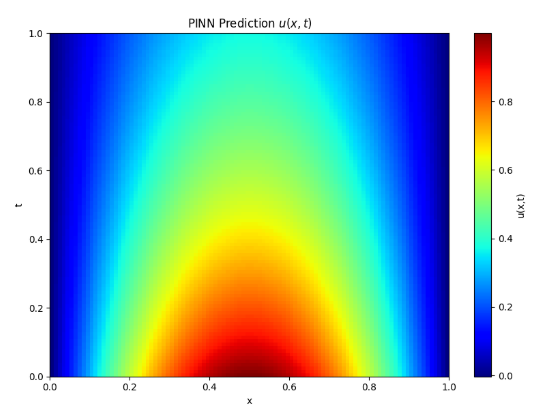
\includegraphics[width=\linewidth]{pres_PINN.png}
        \end{minipage}
        \hfill
        \begin{minipage}{0.48\textwidth}
            \centering
            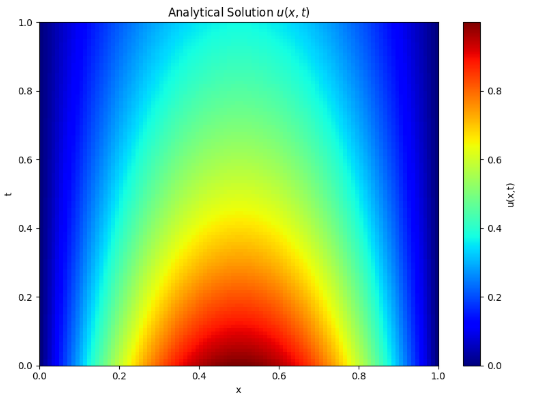
\includegraphics[width=\linewidth]{pres_analytical.png}
        \end{minipage}
    \end{figure}
\end{frame}

\begin{frame}{Crank-Nicolson vs Analytical Solution}
    \begin{figure}[H]
        \centering
        \begin{minipage}{0.48\textwidth}
            \centering
            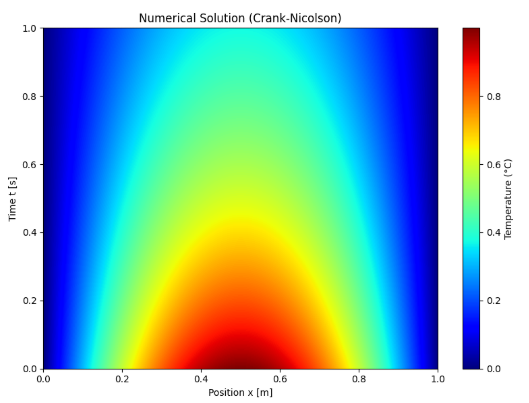
\includegraphics[width=\linewidth]{pres_CN.png}
        \end{minipage}
        \hfill
        \begin{minipage}{0.48\textwidth}
            \centering
            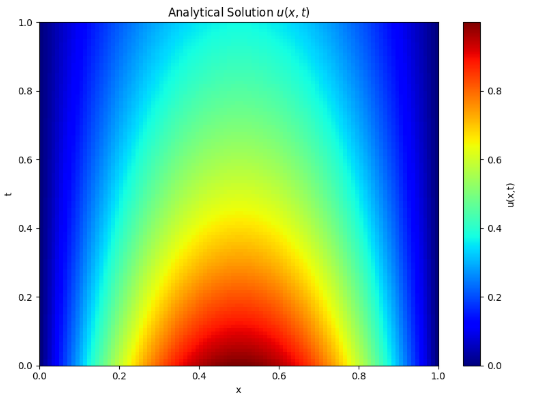
\includegraphics[width=\linewidth]{pres_analytical.png}
        \end{minipage}
    \end{figure}
\end{frame}

\begin{frame}{PINN Error vs Crank Nicolson Error}
    \begin{figure}[H]
        \centering
        \begin{minipage}{0.48\textwidth}
            \centering
            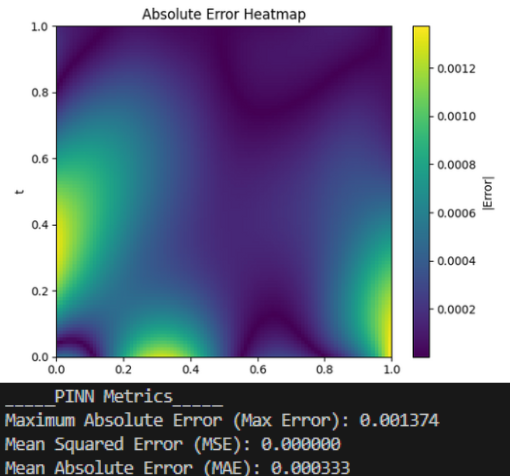
\includegraphics[width=\linewidth]{PINN pres err.png}
        \end{minipage}
        \hfill
        \begin{minipage}{0.48\textwidth}
            \centering
            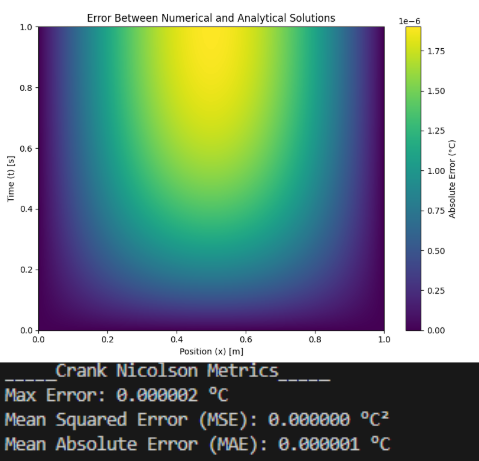
\includegraphics[width=\linewidth]{CN pres ERR.png}
        \end{minipage}
    \end{figure}
\end{frame}

\begin{frame}{Conclusions}
    \begin{itemize}
        \item Both the PINN and Numerical Method did an exceptional job at approximating the solution
        \item Overall, the numerical methods error metrics were better than the PINNs
        \item The numerical method was implemented more efficiently, and both were ran on the CPU
        \item The error maps show clear patterns for the numerical method, and unpredictable patterns for the PINN
        \item The PINN graphed better than the numerical method because of discretization
    \end{itemize}
\end{frame}


\end{document}
